%!TEX root = report.tex

\subsection{Intrinsic Calibration}
\label{sec:intrinsic}

Every camera is characterised by what is called its \textit{intrinsic parameters}. They consist of the focal width and height, $f_x$ and $f_y$, the principal point $c_x$,$c_y$ which is usually at the image center. These parameters are grouped in the camera matrix $C$:

\begin{align}
    C &= \begin{bmatrix}
        f_x & 0 & c_x \\
        0 & f_y & c_y \\
        0 & 0 & 1 \\
    \end{bmatrix} 
\end{align}

Furthermore, every camera creates some radial and tangential distortion in the images which needs to be taken into account. 
If $x'$ and $y'$ are the undistorted image points normalized with $z$ such that $z'=1$ and centered around the principal point $c_x$ and $c_y$, and $r^2=x'^2+y'^2$,
then the distorted points $x''$ and $y''$ can be modelled using Brown-Conrady's decentering distortion model \cite{Brown1966}, \cite{Conrady1919}. 
\begin{align}
    x'' &= x' k(r) + (2p_1 x' y' + p_2(r^2 + 2x'^2))(1+p_3r^2+p_4r^4 + \cdots) \\
    y'' &= y' k(r) + (p_1(r^2+2y'^2) + 2p_2x'y')(1+p_3r^2+p_4r^4 + \cdots) \\
    with \quad k(r) &= 1+k_1r^2+k_2r^4 + \cdots
\end{align}
The distortion coefficients are indifferent to the camera resolution \cite{calib3d}, only the focal width and height and the principal point have to be scaled appropriately. To reduce imprecisions due to scaling, a recalibration was done every time the camera resolution was changed.

An algorithm for finding the intrinsic parameters including the radial distortion coefficients was suggested by Zhang \cite{Zhang2000}. 
Its implementation in the Matlab Camera Calbiration Toolbox added an estimation algorithm for two tangential distortion coefficients. \cite{MTB}
The OpenCV implementation used in this project is based on the Matlab Toolbox. It is implemented for the first 6 radial distortion coefficients $r_i$ and the first 2 tangential distortion coefficients $p_i$ \cite{calib3d}.
% QUESTION: where does the opencv implementation come from??
%$\quad k(r) &=\frac{1+k_1r^2+k_2r^4+k_3r^6}{1+k_4r^2+k_5r^4+k_6r^6} $


%\begin{lstlisting}[caption=Listing]
%\end{lstlisting}

%\begin{figure}[H]
%	\centering
%	\begin{subfigure}[b]{0.49\linewidth}
%		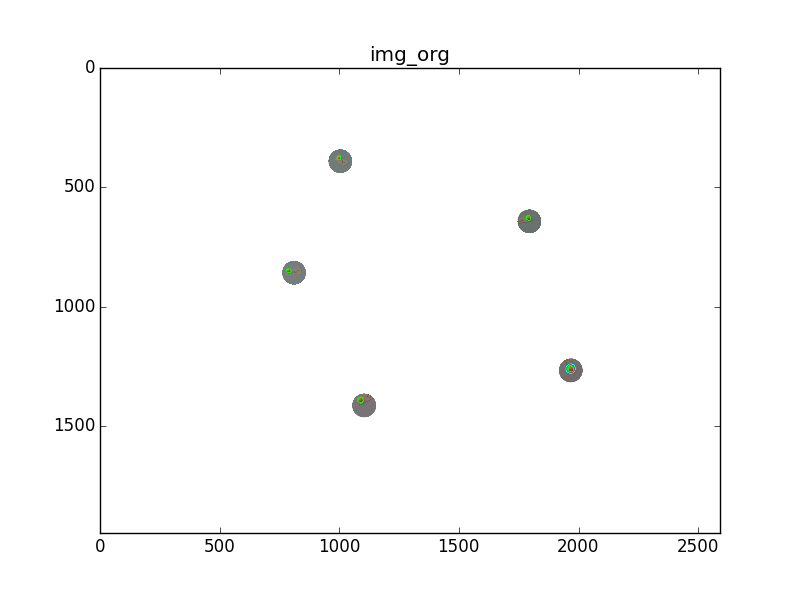
\includegraphics[width=\linewidth]{../files/img_org139.png}
%		\caption{Regions of interest chosen by user and extracted colors}
%		\label{feat_step0}
%	\end{subfigure}
%	\begin{subfigure}[b]{0.49\linewidth}
%		\includegraphics[width=\linewidth]{../files/img_h139.png}
%		\caption{\textit{Hue} representation of original image}
%		\label{feat_step1}
%	\end{subfigure}
%	\begin{subfigure}[b]{0.49\linewidth}
%		\includegraphics[width=\linewidth]{../files/img_s139.png}
%		\caption{\textit{Saturation} representation of original image}
%		\label{feat_step2}
%	\end{subfigure}
%	\begin{subfigure}[b]{0.49\linewidth}
%		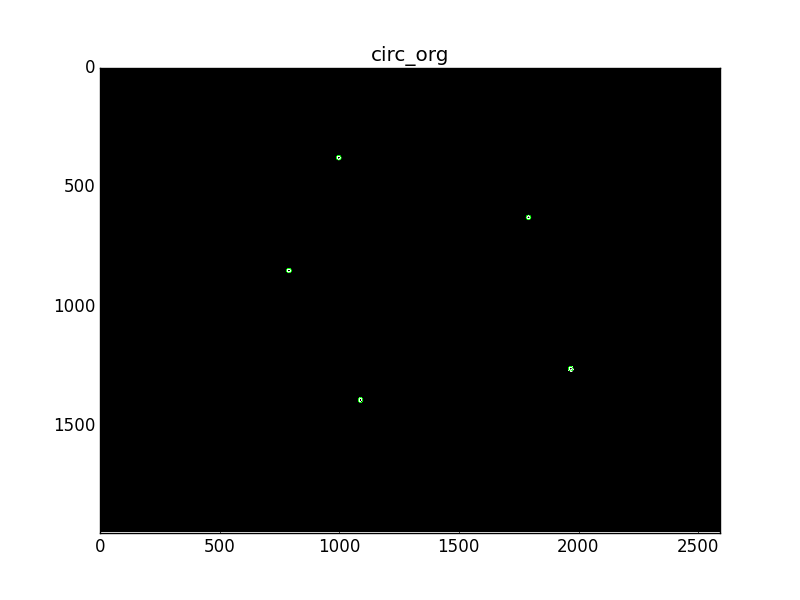
\includegraphics[width=\linewidth]{../files/circ_org139.png}
%		\caption{Regions of interest chosen by user and extracted colors}
%		\label{feat_step3}
%	\end{subfigure}
%	
%	
%	\begin{subfigure}[b]{0.49\linewidth}
%		\includegraphics[width=\linewidth]{../files/zdot_RefTrackNL.png}
%	\end{subfigure}
%	\begin{subfigure}[b]{0.49\linewidth}
%		\includegraphics[width=\linewidth]{../files/speeds_RefTrackNL.png}
%	\end{subfigure}
%	\begin{subfigure}[b]{0.49\linewidth}
%		\includegraphics[width=\linewidth]{../files/xyz_RefTrackNL.png}
%	\end{subfigure}
%	\caption{Procedure for feature extraction} 
%\end{figure}
